\documentclass{article}
\usepackage[utf8]{inputenc}
\usepackage{geometry}
\usepackage{graphicx}
\geometry{a4paper, margin=1in}

\title{Manual de Usuario}
\author{}
\date{}

\begin{document}

\maketitle

\section*{Introducción}
El presente informe tiene como objetivo documentar el desarrollo e implementación del software, proporcionando una descripción detallada de sus funcionalidades, 
requisitos y procedimientos de uso. Este documento está dirigido a usuarios finales, administradores y cualquier persona encargada de la operación del sistema. A 
través de este manual, se busca facilitar la instalación, configuración y uso eficiente de la aplicación, asegurando una experiencia óptima y reduciendo posibles 
incidencias durante su utilización.

\section*{Objetivo del Proyecto}

El presente proyecto tiene como finalidad desarrollar una aplicación web para la gestión y control del consumo eléctrico en diversas sucursales de una empresa. El 
sistema proporcionará información detallada sobre el uso de energía en cada instalación, permitiendo a los responsables tomar decisiones estratégicas para la 
optimización de los recursos energéticos y la reducción del consumo eléctrico.

A través de esta plataforma, los usuarios podrán visualizar resúmenes del consumo energético de todas las sucursales. Se establecerán distintos niveles de acceso, 
donde los administradores especializados y gerentes tendrán el control total sobre la configuración de los centros de trabajo y las políticas de consumo energético. 
Entre sus funciones, estos usuarios podrán agregar y gestionar centros de trabajo, configurar límites de consumo y generar reportes avanzados.

Además, se implementará una funcionalidad que permitirá calcular el costo total del consumo eléctrico en cada sucursal mediante una fórmula predefinida, la cual 
podrá ser ajustada por los administradores especializados según las necesidades específicas de cada centro de trabajo. La plataforma almacenará información detallada 
sobre los equipos eléctricos, sus características técnicas y su impacto en el consumo energético, facilitando un análisis más preciso y promoviendo la eficiencia en 
el uso de la energía.

El sistema ofrecerá herramientas para consultar datos históricos de consumo, identificar tendencias, predecir consumos futuros y evaluar el impacto de nuevas políticas 
de eficiencia energética. Asimismo, contará con la capacidad de generar reportes en distintos formatos y emitir alertas en caso de sobrepasar los límites de consumo 
establecidos.


\section*{Requerimientos Técnicos}

La aplicación web está diseñada para funcionar en una variedad de navegadores modernos y sistemas operativos.  Las características mínimas de la máquina o red donde se 
ejecutará la aplicación son:

\begin{itemize}
    \item \textbf{Navegador:}  Chrome (versión reciente), Firefox (versión reciente), Safari (versión reciente), Edge (versión reciente).
    \item \textbf{Sistema Operativo:} Windows 10 o superior, macOS 10.15 o superior, Linux (distribuciones modernas).
    \item \textbf{Conexión a Internet:}  Se requiere una conexión a internet estable para el correcto funcionamiento de la aplicación.  La velocidad mínima recomendada es de 5 Mbps.
    \item \textbf{Resolución de pantalla:}  Se recomienda una resolución de pantalla mínima de 1366x768 píxeles.
\end{itemize}


\section*{Requerimientos de Software}

Para ejecutar la aplicación, no se requiere la instalación de ningún software adicional en el cliente (el usuario final que usa el navegador web).  La aplicación funciona completamente en el navegador web.   El servidor que aloja la aplicación requerirá un servidor web (como Apache o Nginx), una base de datos (como MySQL o PostgreSQL), y un entorno de ejecución para el lenguaje de programación usado en el backend de la aplicación.  Estos son requisitos del administrador del sistema, no del usuario final.

\section*{Instalación de la Aplicación}

La aplicación se ejecuta directamente en el navegador web. No hay necesidad de instalar ningún software en la máquina del usuario.  Para acceder a la aplicación, simplemente navegue hasta la dirección URL proporcionada por el administrador del sistema.


\section{Opciones del Sistema}
Este manual describe las funcionalidades del sistema de gestión del consumo eléctrico.  Le guiará a través de las diferentes opciones disponibles.

\subsection{Acceso al Sistema}

\subsubsection{Autenticación}
Para acceder al sistema, deberá autenticarse introduciendo su nombre de usuario y contraseña en la pantalla de inicio de sesión, a continuación se muestra un ejemplo de entrada y posible respuesta.

\begin{figure}[h!]
    \centering
    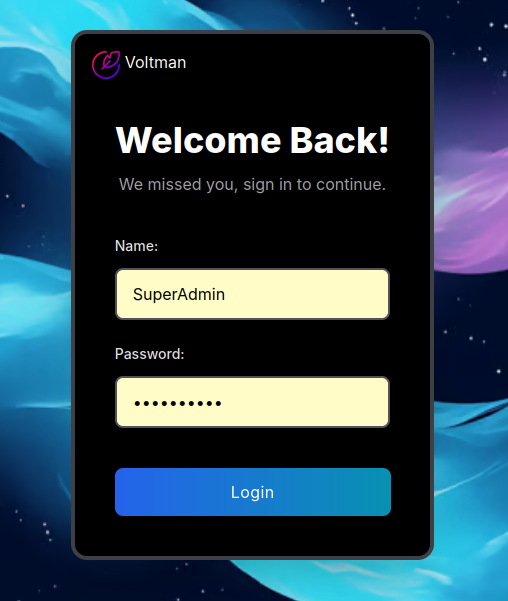
\includegraphics[width= 6cm]{login_page.png}
    \caption{Imagen de la página de Login.}
\end{figure}

Se inserta el username y password para luego tocar en el botón de login y esperar una respuesta, en caso e haber errores se mostrarán algunos detalles en una pequeña ventana.

\begin{figure}[h!]
    \centering
    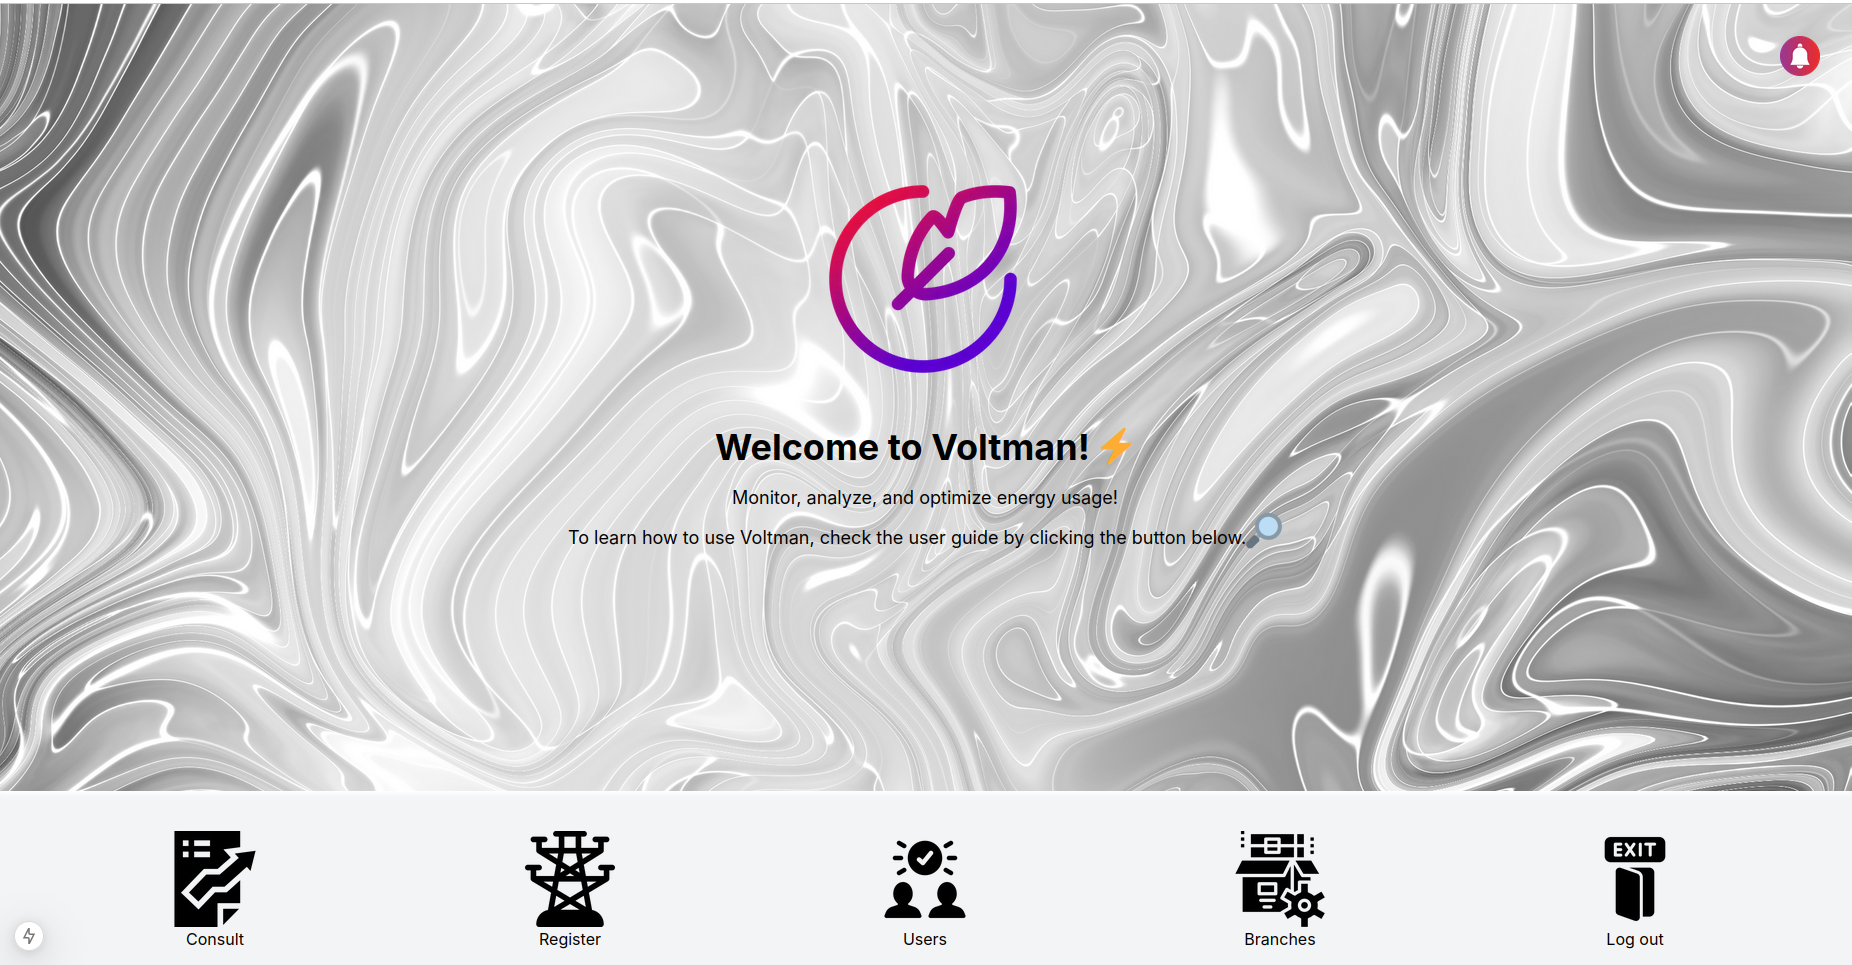
\includegraphics[width= 12cm]{home_page.png}
    \caption{Respuesta, redireccionamiento a la página de Home.}
\end{figure}


\subsection{Opciones Principales}
\subsubsection{Gestión de Usuarios}
Esta sección permite la administración de cuentas de usuario a la cual solo tienen acceso los administradores de centro:

\begin{itemize}
    \item \textbf{Listar:} Muestra una lista con los usuarios registrados.
    
    \begin{figure}[h!]
        \centering
        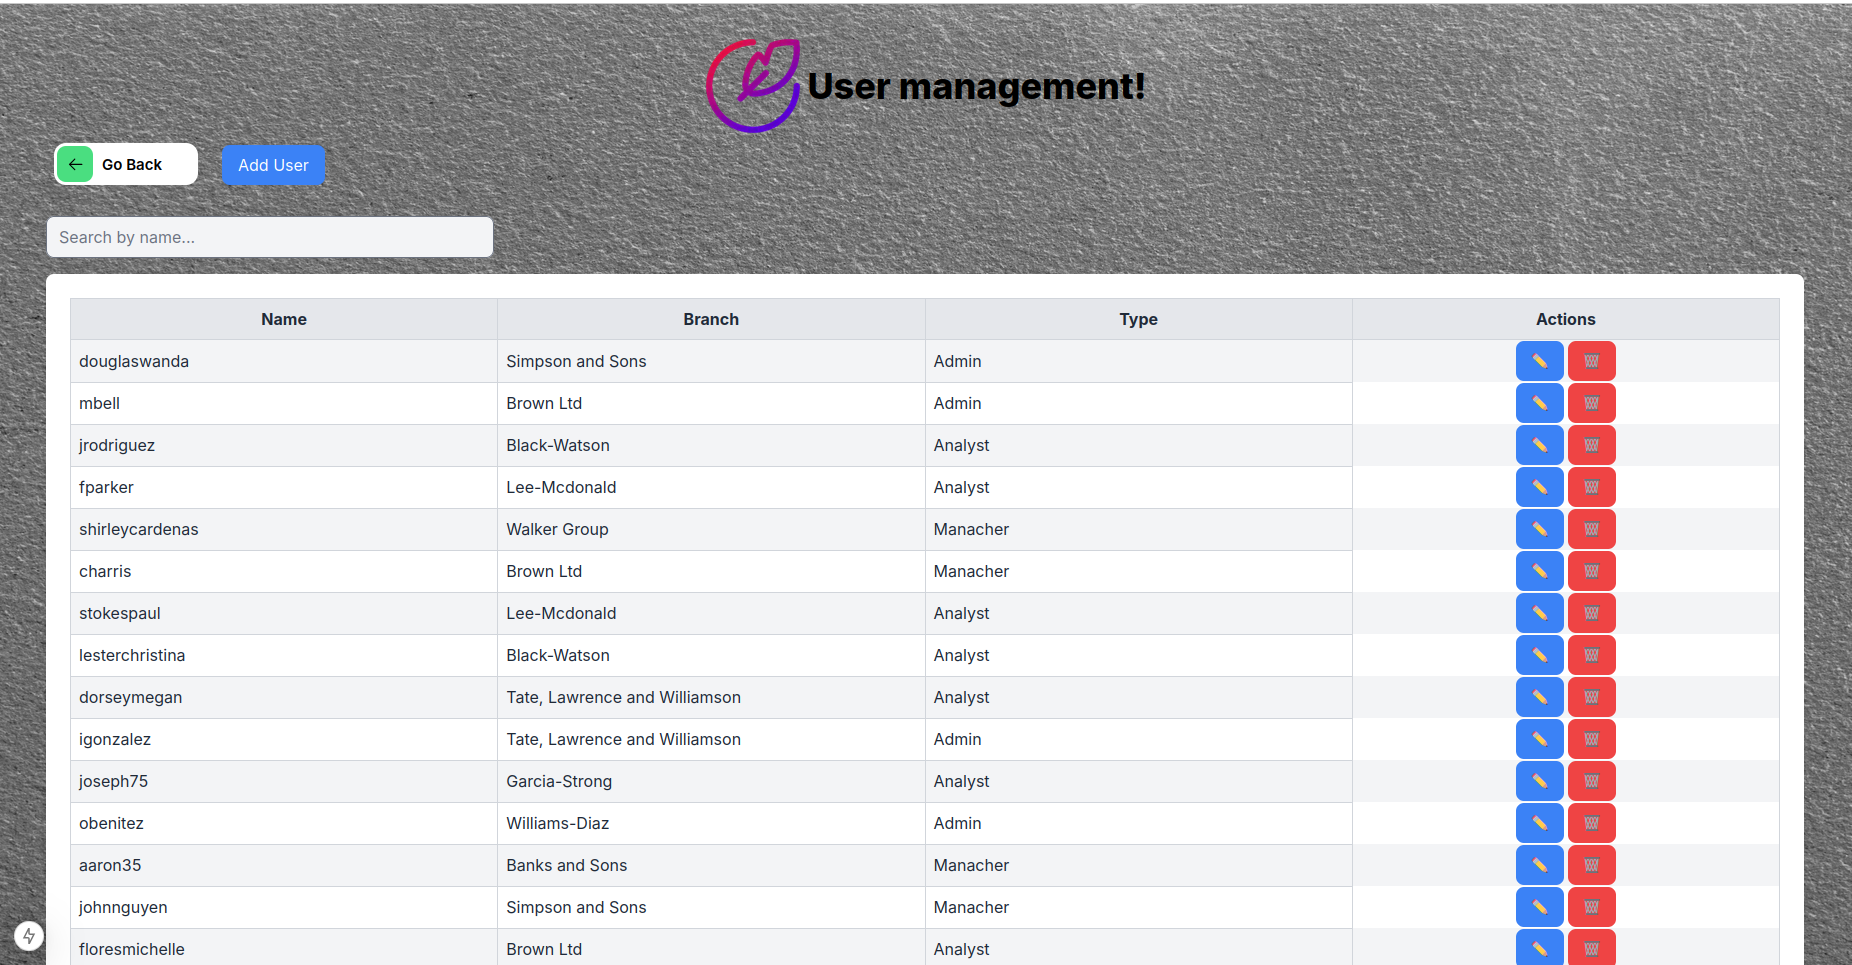
\includegraphics[width= 12cm]{listar_users.png}
        \caption{Lista con usuarios registrados en el sistema}
    \end{figure}

    \item \textbf{Agregar:} Permite crear una nueva cuenta de usuario. Se deben rellenar todos los datos correspondientes.
    
    \begin{figure}[h!]
        \centering
        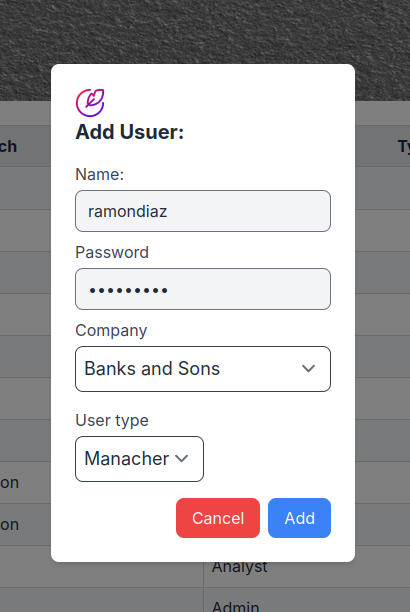
\includegraphics[width= 5cm]{add_user.png}
        \caption{Ejemplo de cómo agregar un usuario}
    \end{figure}

    \begin{figure}[h!]
        \centering
        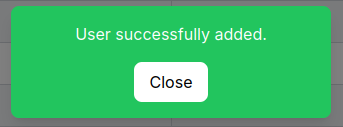
\includegraphics[width= 5cm]{add_user_response.png}
        \caption{Ejemplo de posible respuesta al agregar un nuevo usuario}
    \end{figure}  

    \item \textbf{Editar:} Permite modificar la información de un usuario existente. Se deben rellenar los datos correspondientes, el administrador debe conocer la 
    contraseña del usuario para poder editar su información correctamente, en caso contrario saldrá una ventana con información sobre el error.
    
    \begin{figure}[h!]
        \centering
        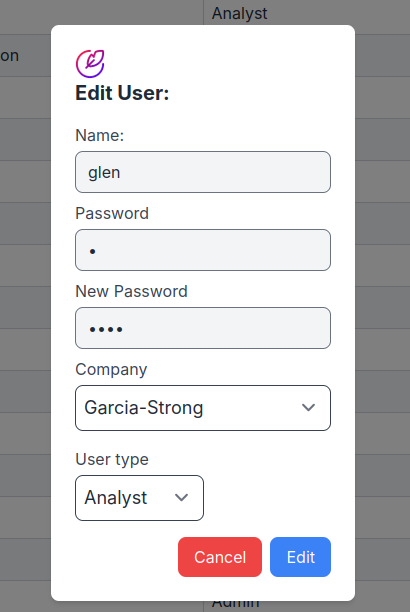
\includegraphics[width= 5cm]{edit_user.png}
        \caption{Ejemplo de cómo editar un usuario.}
    \end{figure}

    \item \textbf{Eliminar:} Permite eliminar una cuenta de usuario. Se debe hacer click en el botón rojo.
    
    \begin{figure}[h!]
        \centering
        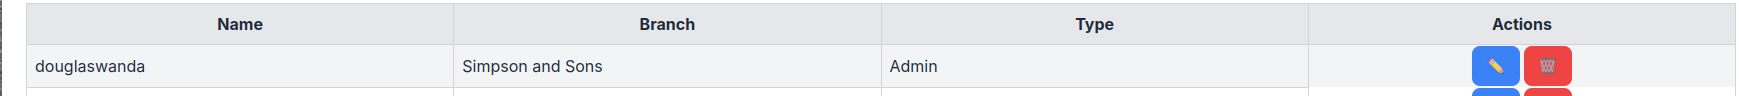
\includegraphics[width= 16cm]{delete_user.png}
        \caption{Ejemplo de como eliminar un usuario.}
    \end{figure}

\end{itemize}

\subsubsection{Gestión de Sucursales}
Esta sección gestiona la información de las sucursales. A esta página solo tienen acceso los administradores y jefes de centro. Se presiona el botón Branches en la página de Home (Ver Figura 2).

\begin{itemize}
    \item \textbf{Acceder a información:} Muestra detalles de una sucursal seleccionada. 
    \item \textbf{Editar información:} Permite modificar la información de una sucursal, se presiona el botón Save en Branch info. (Ver Figura 8)
    \item \textbf{Agregar sucursal:} Permite crear un nuevo registro de sucursal. Solo el SuperAdministrador tiene permiso para crear o eliminar una sucursal. 
    Se presiona el botón Add (Ver Figura 8) y se rellena el formulario correspondiente.
    \item \textbf{Eliminar sucursal:} Permite eliminar un registro de sucursal presionando el botón Delete (Ver Figura 8). Esto solo es posible si la sucursal seleccionada no cuenta con áreas dentro de ella.
\end{itemize}

\begin{figure}[h!]
    \centering
    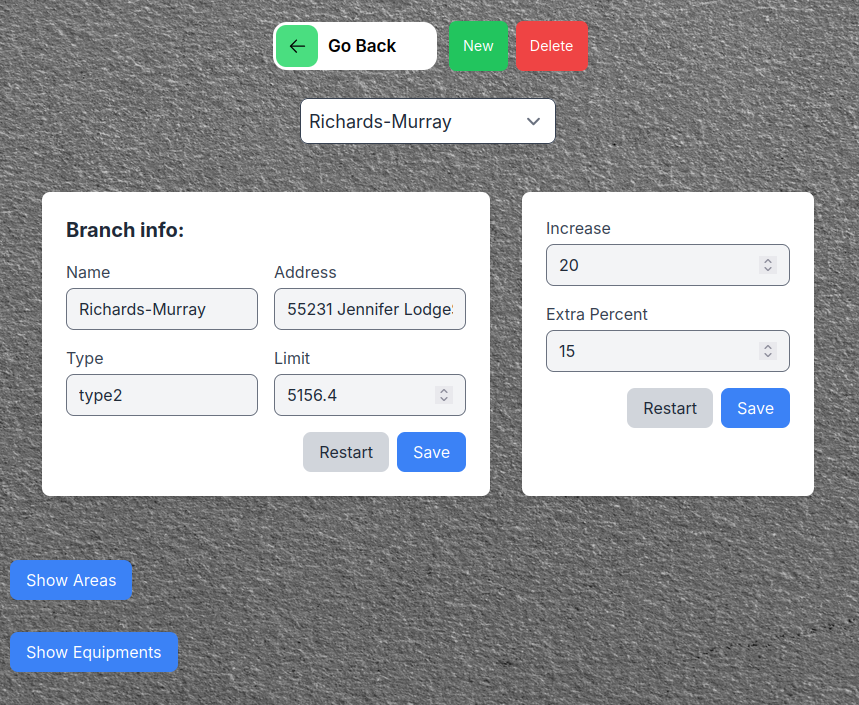
\includegraphics[width= 12cm]{branch_page.png}
    \caption{Imagen de página de sucursales.}
\end{figure}


\subsubsection{Gestión de Áreas}
Esta sección gestiona las áreas dentro de una sucursal. Tanto los administradores como jefes de centro pueden realizar estas operaciones.

\begin{itemize}
    \item \textbf{Listar áreas:} Muestra una lista de las áreas dentro de una sucursal seleccionada. Se presiona el botón Show Areas (ver Figura 8).
    \item \textbf{Agregar:} Permite añadir una nueva área. Se presiona el botón Add Área (Ver Figura 9) y se rellena el respectivo formulario.
    \item \textbf{Eliminar:} Permite eliminar un área. Se presiona el botón Delete ubicado a la parte derecha de la información de cada Área(Ver Figura 9).
    \item \textbf{Editar:} Permite modificar la información de un área. Se presiona el botón Edit ubicado a la parte derecha de la información de cada Área(Ver Figura 9).
    
    \begin{figure}[h!]
        \centering
        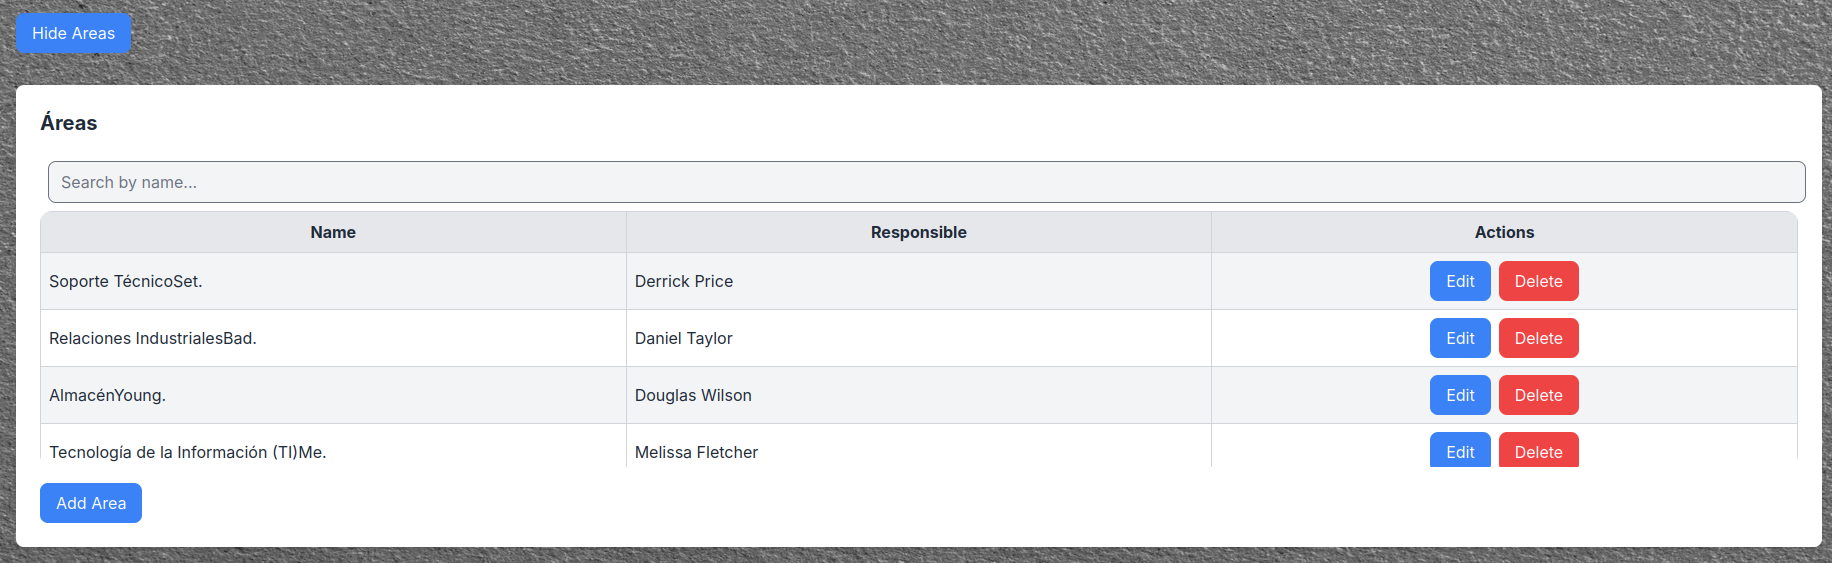
\includegraphics[width= 14cm]{list_area.png}
        \caption{Ejemplo de listar Áreas.}
    \end{figure}

    \begin{figure}[h!]
        \centering
        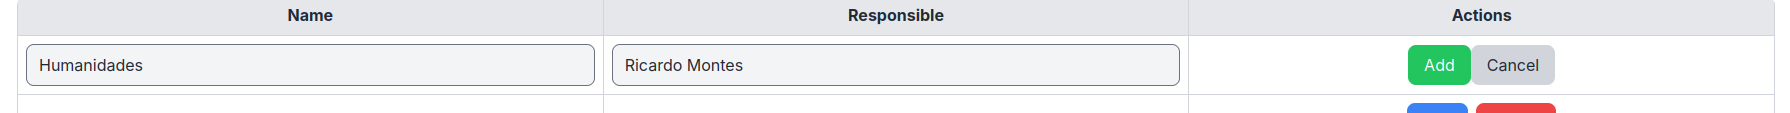
\includegraphics[width= 14cm]{add_area.png}
        \caption{Ejemplo de Agregar un Área.}
    \end{figure}

    \begin{figure}[h!]
        \centering
        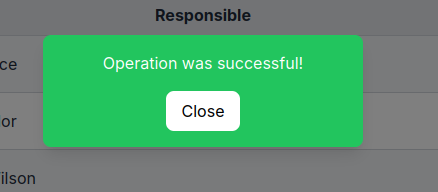
\includegraphics[width= 4cm]{response.png}
        \caption{Respuesta luego de agregar un Área.}
    \end{figure}

\end{itemize}

\subsubsection{Gestión de Equipos}
Esta sección gestiona los equipos que consumen energía:

\begin{itemize}
    \item \textbf{Listar equipos:} Muestra una lista de los equipos en una sucursal. Presiona el botón Show Equipments(Ver Figura 8).
    \item \textbf{Agregar:} Permite añadir un nuevo equipo. Se presiona en el botón New Equipment (Ver Figura 12) y se rellena el respectivo formulario (Ver Figura 13).
    \item \textbf{Eliminar:} Permite eliminar un equipo. Se presiona el botón Delete que se encuentra en el extremo derecho de la información de cada equipo(Ver Figura 12).
    \item \textbf{Editar:} Permite modificar la información de un equipo. Se presiona el botón Edit que se encuentra en el extremo derecho de la información de cada 
    equipo(Ver Figura 12). Y se rellena el respectivo formulario que es idéntico al formulario de Add Equipment (Ver Figura 13).
    
    \begin{figure}[h!]
        \centering
        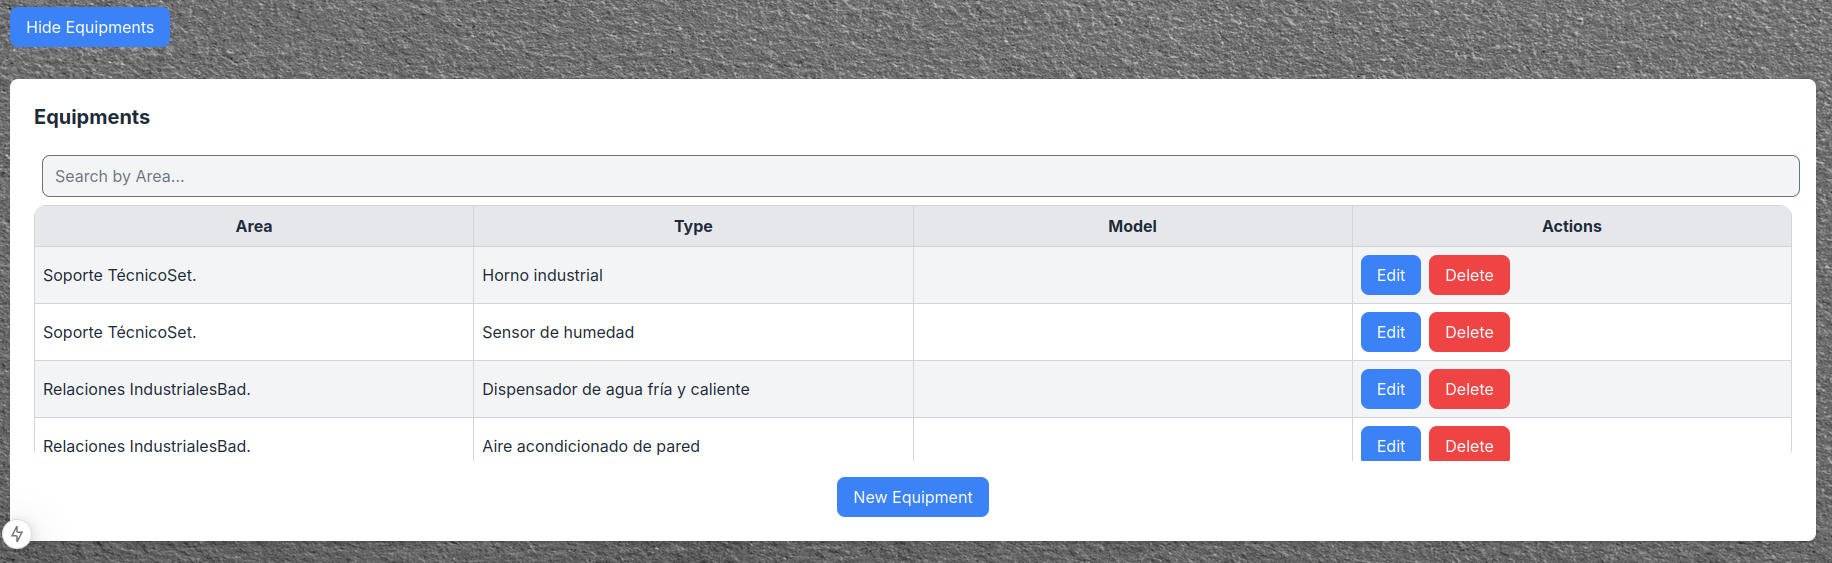
\includegraphics[width= 14cm]{list_equipments.png}
        \caption{Ejemplo de listar Equipments.}
    \end{figure}

    \begin{figure}[h!]
        \centering
        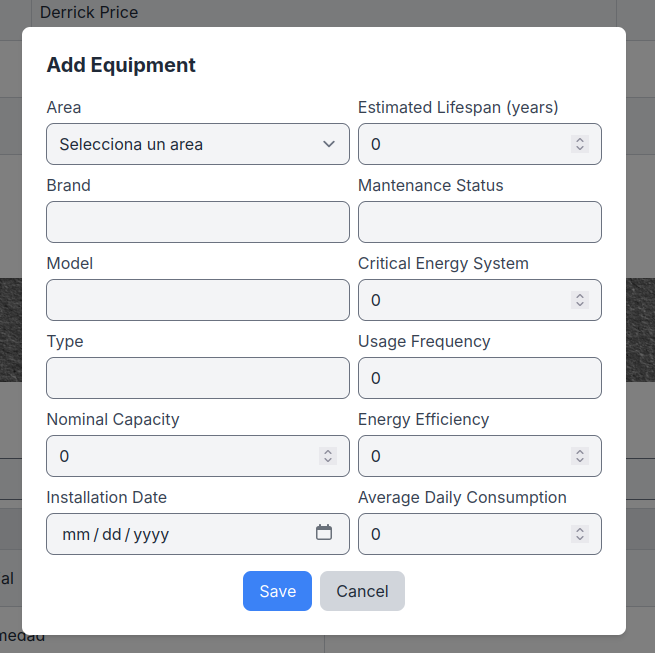
\includegraphics[width= 8cm]{add_equipment.png}
        \caption{Formulario para agregar un equipo.}
    \end{figure}

\end{itemize}

\subsubsection{Registrar Consumos}
Permite registrar el consumo diario de energía de una sucursal.Solo los jefes de centro tienen acceso a esta página. Se presiona en el botón de Register de la página de Home (Ver Figura 2) para acceder a la página correspondiente.
Como se observa, hay dos botones fundamentales, Register para registrar consumo y Add para agregar un nuevo formulario para guardar otro registro.
\begin{figure}[h!]
    \centering
    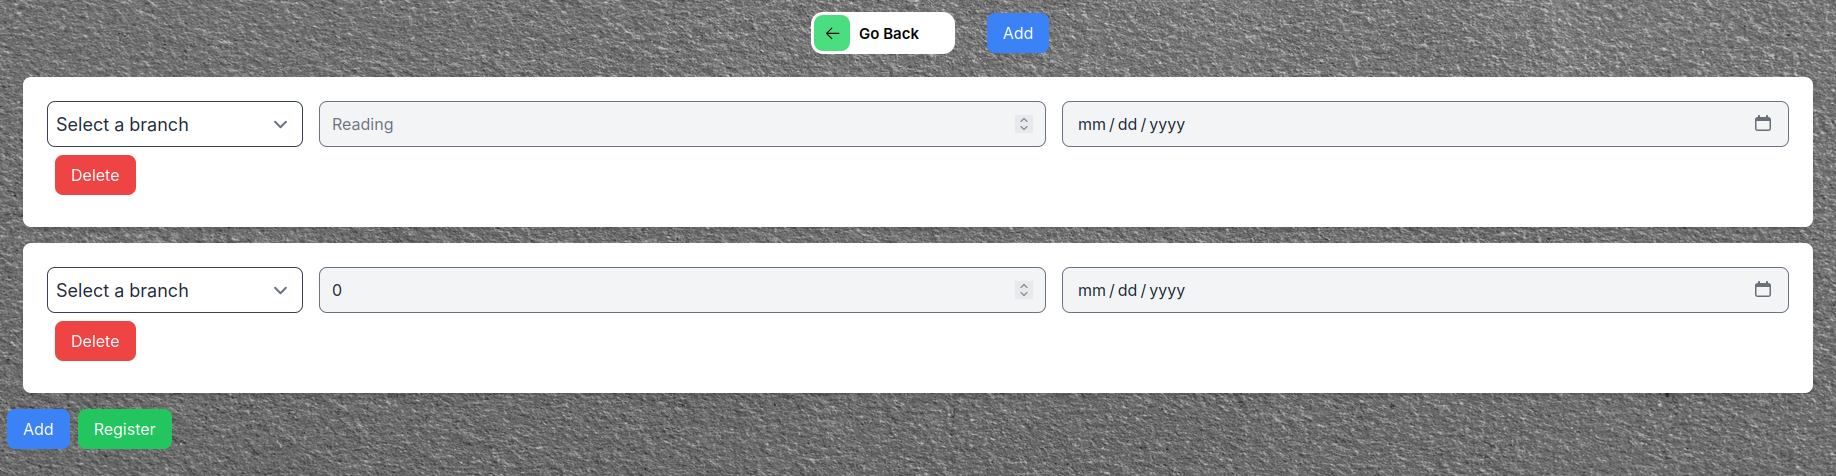
\includegraphics[width= 14cm]{register_consume.png}
    \caption{Página de Registro de Consumo.}
\end{figure}

\subsubsection{Editar Fórmula de Costos}
Permite modificar la fórmula de cálculo de costos de consumo de energía. Los valores que se pueden modificar son Increase y Extra Percent, el único usuario autorizado para 
realizar esta operación es el administrador (Ver Figura 8). Se guardan los cambios tras tocar el botón Save.

\subsubsection{Consultas}
Esta sección ofrece diferentes opciones de consulta. Todos los usuarios tienen acceso a esta página. Para acceder se debe tocar el botón Consult en la página 
Home (ver Figura 2). A continuación se procede a seleccionar la consulta que sea de interés. (Ver Figura 15).

\begin{figure}[h!]
    \centering
    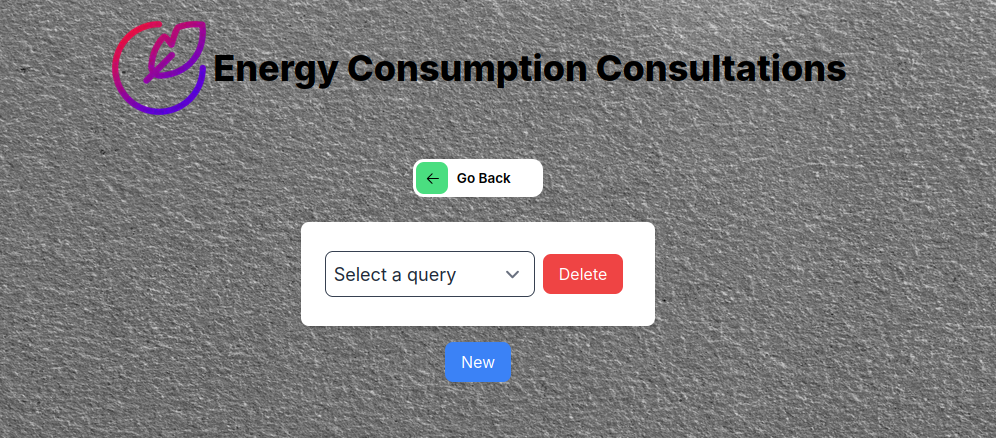
\includegraphics[width= 10cm]{consult_page.png}
    \caption{Página de Consultas.}
\end{figure}

\begin{enumerate}
    \item Consultar consumo en un rango de fechas. Se rellena el formulario correspondiente y se presiona el botón Consult ubicado en la parte inferior del formulario.(Figura 16).
    \begin{figure}[h!]
        \centering
        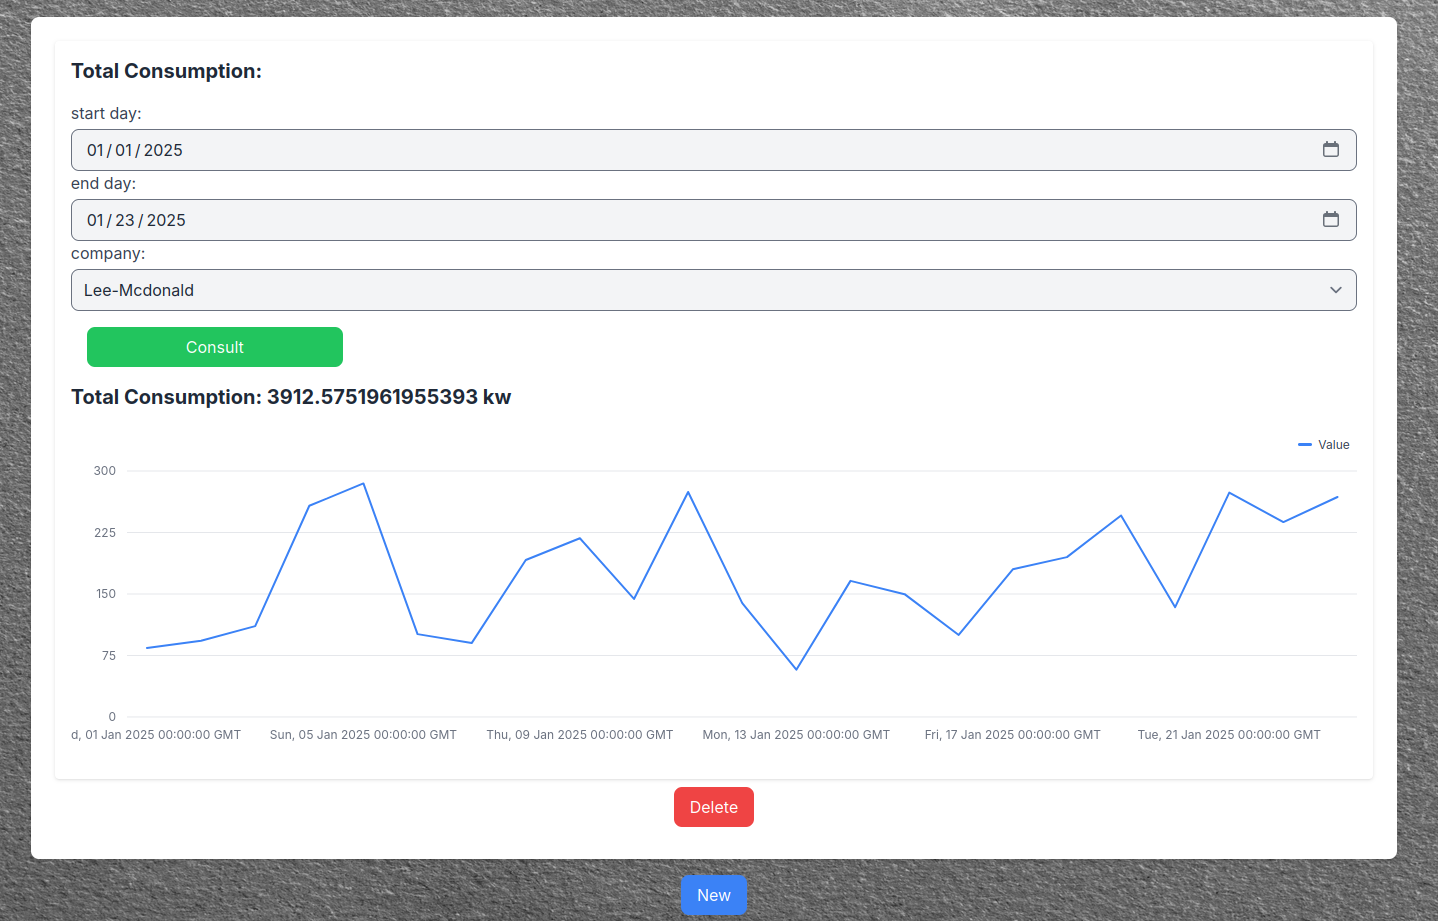
\includegraphics[width= 14cm]{total_consumption.png}
        \caption{Consumo Total de una Sucursal en Rango de Fechas.}
    \end{figure}
    \item Promedios mensuales de los últimos 3 años. Se rellena el formulario correspondiente y se presiona el botón Consult ubicado en la parte inferior del formulario.(Figura 17).
    \begin{figure}[h!]
        \centering
        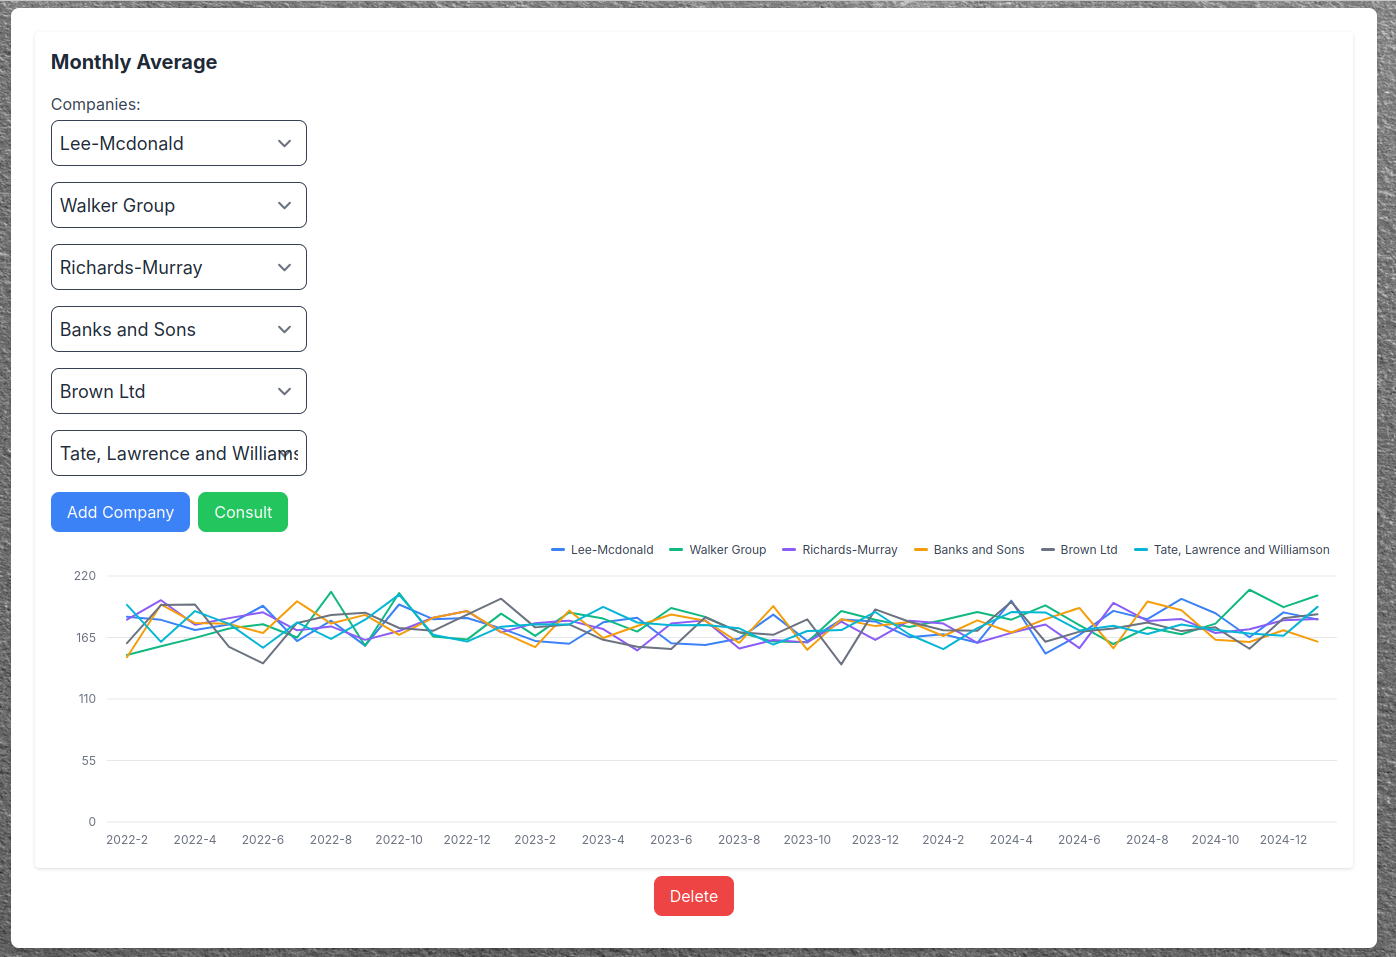
\includegraphics[width= 14cm]{monthly_average.png}
        \caption{Gráfico de Promedios Mensuales de algunas Sucursales en los últimos 3 años.}
    \end{figure}
    \item Predecir consumo para el próximo trimestre. Se rellena el formulario correspondiente y se presiona el botón Consult ubicado en la parte inferior del formulario.(Figura 18).
    \begin{figure}[h!]
        \centering
        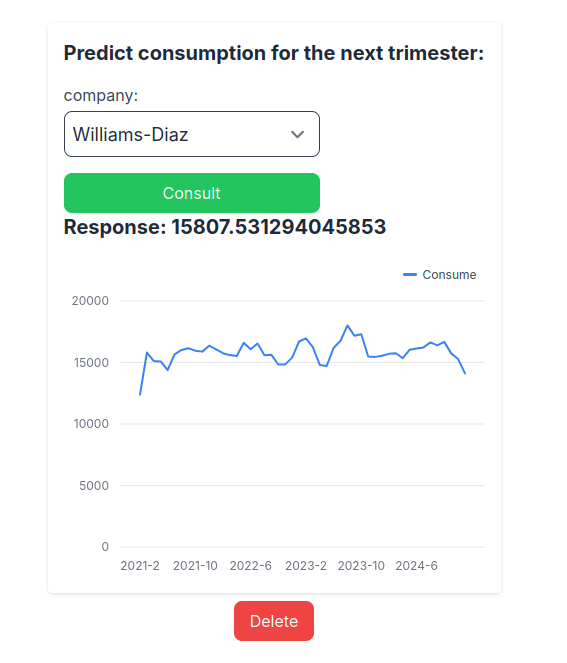
\includegraphics[width= 10cm]{predict_consume.png}
        \caption{Predecir consumo para el próximo trimestre basado en datos históricos.}
    \end{figure}
    \item Mostrar información de equipos dentro de un área específica.Se rellena el formulario correspondiente y se presiona el botón Consult ubicado en la parte inferior del formulario.(Figura 19).
    \begin{figure}[h!]
        \centering
        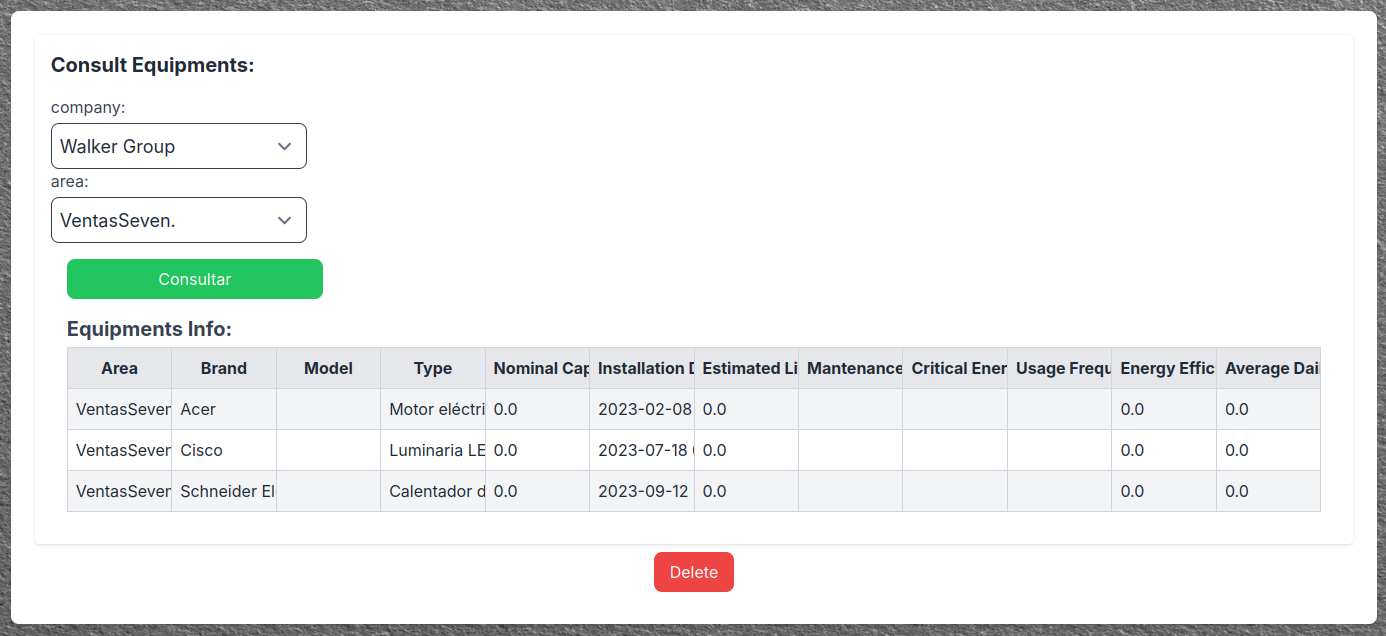
\includegraphics[width= 14cm]{consult_equipments.png}
        \caption{Información de Equipos dentro de un Área específica.}
    \end{figure}
    \item Listar sucursales que excedieron el límite de consumo.Se rellena el formulario correspondiente y se presiona el botón Consult ubicado en la parte inferior del formulario.(Figura 20).
    \begin{figure}[h!]
        \centering
        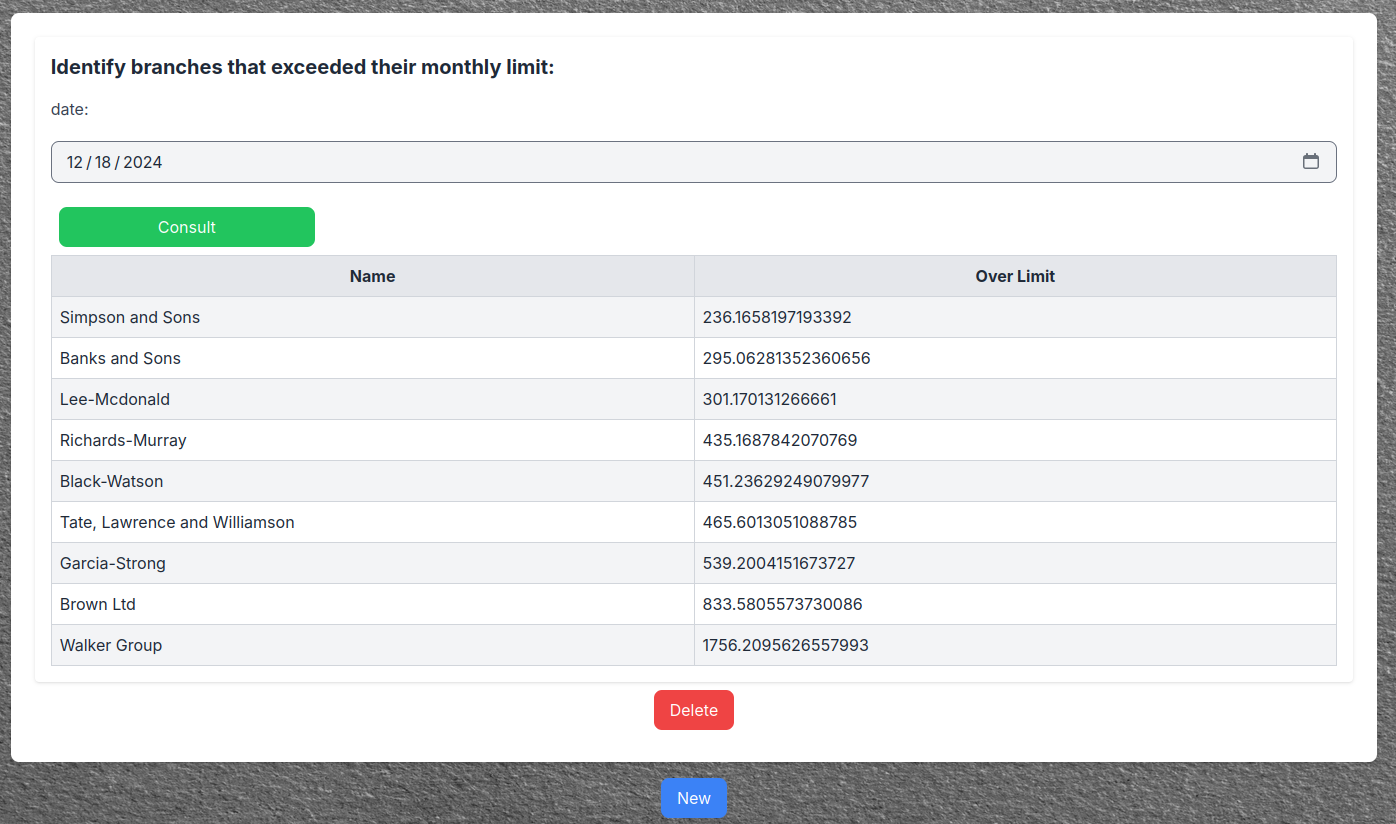
\includegraphics[width= 14cm]{identify_branches.png}
        \caption{Ejemplo de Sucursales que excedieron su límite en el mes de Diciembre 2024.}
    \end{figure}
    % \item Comparar eficiencia energética antes y después de una fecha.
    % \begin{figure}[h!]
    %     \centering
    %     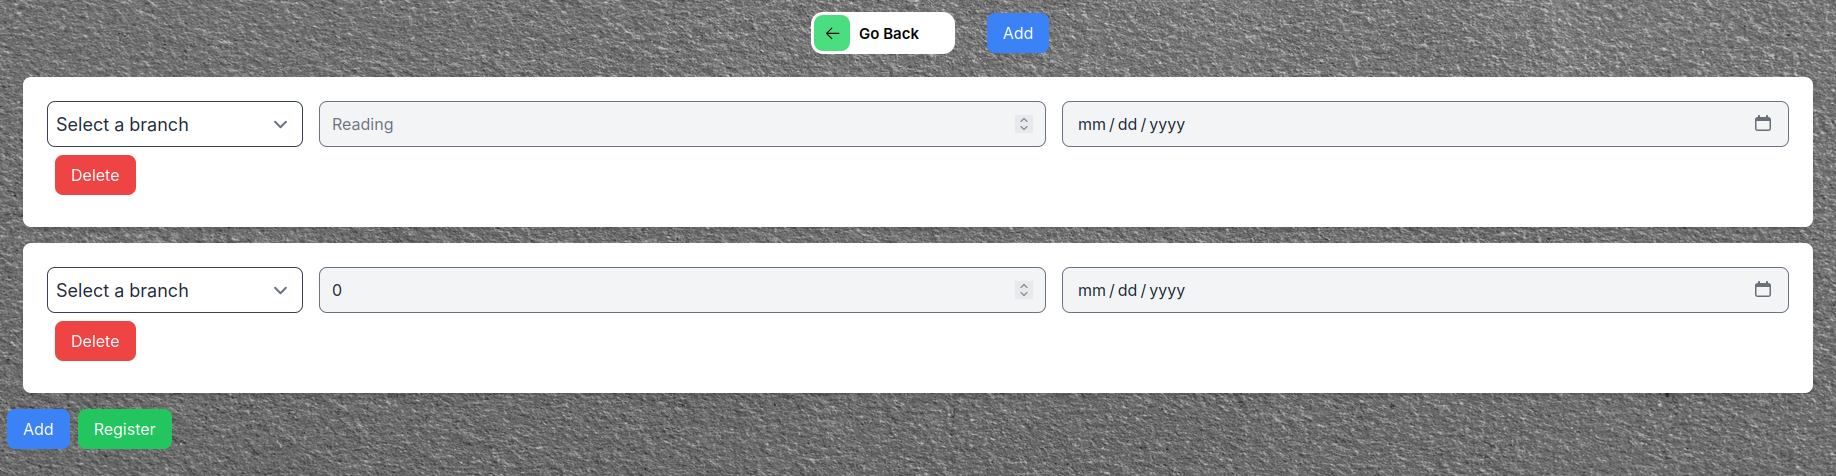
\includegraphics[width= 14cm]{register_consume.png}
    %     \caption{Página de Registro de Consumo.}
    % \end{figure}
    \item Exportar información a PDF.
\end{enumerate}

\end{document}